%\documentclass[trans]{beamer}
\documentclass[9pt]{beamer}

% Try the class options [notes], [notes=only], [trans], [handout],
% [red], [compress], [draft], [class=article] and see what happens!

% Copyright 2003 by Till Tantau <tantau@users.sourceforge.net>.
%
% This program can be redistributed and/or modified under the terms
% of the LaTeX Project Public License Distributed from CTAN
% archives in directory macros/latex/base/lppl.txt.

% For a green structure color use:
%\colorlet{structure}{green!50!black}

%%%%%%%%%% User macros%%%%%%%%%%%
\newcommand{\mypurple}[1]{{\color[rgb]{0.7,0,0.8}#1}}
\newcommand{\myred}  [1] {{\color{red}#1}}
\newcommand{\myblue} [1] {{\color{blue}#1}}
\newcommand{\mygreen}[1] {{\color[rgb]{0,0.5,0}#1}}
\newcommand{\Nat}{\mathbb{N}}
\def\sla  {\!\!\!\slash}
%%%%%%%%%%%%%%%%%%%%%%%%%%%%%%%%%
\mode<article> % only for the article version
{
  \usepackage{beamerbasearticle}
  \usepackage{fullpage}
  \usepackage{hyperref}
}

%\beamertemplateshadingbackground{red!10}{blue!10}
%\beamertemplateshadingbackground{blue!10}{blue!10}

%\usepackage{beamerthemeshadow}

\usepackage{pgf,pgfarrows,pgfnodes,pgfautomata,pgfheaps,pgfshade}
\usepackage{amsmath,amssymb}
\usepackage[latin1]{inputenc}
\usepackage{colortbl}
\usepackage[english]{babel}
%\usepackage{verbatim}
%\usepackage{listings}
\usepackage[procnames]{listings}

%\usepackage{lmodern}
\usepackage[T1]{fontenc} 

\usepackage{times}

% for code colouring
\include{pythonlisting}
\include{cpplisting}
\usepackage{minted}

% Use some nice templates
\beamertemplatetransparentcovereddynamic
\usetheme{Binet}
%\usetheme{Madrid}
%\usetheme{Boadilla}
%\usetheme{Berkeley}
%\usetheme{Rochester}

%\def\command#1{\list{}{\leftmargin=2em\itemindent-\leftmargin\def\makelabel##1{\hss##1}}%
%\item\extractcommand#1@\par\topsep=0pt}
%\def\endcommand{\endlist}
%\def\extractcommand#1#2@{\strut\declare{\texttt{\string#1}}#2}

%
% The following info should normally be given in you main file:
%

\hypersetup{%
  pdftitle={docker-HEP},%
  pdfauthor={Sebastien Binet}
  %pdfsubject={AthenaMP},
  %pdfkeywords={ATLAS,Athena,python,COW,parallelization},
%  pdfpagemode=FullScreen%
}

\title[docker-HEP]{docker \& HEP:\\containerization of applications for development,\\distribution and preservation}
\author[S. Binet]{S\'ebastien~Binet}%\inst{1}
\institute[LAL]{
%  \inst{1}%
  LAL/IN2P3}
\date{2015-04-13}

% \begin{center}
% On behalf of Core people
% \end{center}

\pgfdeclaremask{lal}{lal}
%\pgfdeclaremask{ubp}{UBP-logo}
\pgfdeclareimage[mask=lal,width=2cm]{lal-logo}{lal}
%\pgfdeclareimage[mask=ubp,width=1cm]{ubp-logo}{UBP-logo}

\logo{%
  \vbox{%
    \hbox{\pgfuseimage{lal-logo}}%
  }%
}


\begin{document}
\lstset{language=C++}

\frame{\titlepage
%  \hskip0.44\paperwidth
%  \insertlogo

    \begin{beamercolorbox}[sep=8pt,center]{mylogo}
      \usebeamercolor[fg]{mylogo}\insertlogo
    \end{beamercolorbox}

}

%\section*{Outline}
%\frame{\tableofcontents[part=1]}%,pausesections]}

%\AtBeginSubsection[]
%{
%  \frame<handout:0>
%  {
%    \frametitle{Outline}
%    \tableofcontents[current,currentsubsection]
%  }
%}

\part<presentation>{Main Talk}

%%%%%%%%%%%%%%%%%%%%%%%%%%%%%%%%%%%%%%%%%%%%%%%%%%%%%%%%%%%%%%%%%%%%%%%%%%%%%%%
%%%%%%%%%%%%%%%%%%%%%%%%%%%%%%%%%%%%%%%%%%%%%%%%%%%%%%%%%%%%%%%%%%%%%%%%%%%%%%%
%\section[Outline]{Outline}

% \frame<beamer>{
%   \frametitle{Outline}
%   \begin{columns}
% \begin{column}{0.49\textwidth}
%   \begin{block}{}
%   \tableofcontents
%   \end{block}
% \end{column}
% \end{columns}

% }
%\frame{\partpage}

%%%%%%%%%%%%%%%%%%%%%%%%%%%%%%%%%%%%%%%%%%%%%%%%%%%%%%%%%%%%%%%%%%%%%%%%%%%%%%%
%%%%%%%%%%%%%%%%%%%%%%%%%%%%%%%%%%%%%%%%%%%%%%%%%%%%%%%%%%%%%%%%%%%%%%%%%%%%%%%
\section[mysection]{mysection}

\frame{
  \frametitle{Docker: what is it ?}

  \begin{block}{}
    \begin{itemize}
      \item \myblue{\href{http://www.docker.io/}{\texttt{http://www.docker.io/}}}
      \item an open source project to pack, ship and run any application as a lightweight container
    \end{itemize}
  \end{block}

  \begin{block}{High level description}
    \begin{itemize}
      \item kind of like a \myred{lightweight} VM
      \item runs in its own process space
      \item has its own network interface
      \item can run stuff as \texttt{root}
    \end{itemize}
  \end{block}

  \begin{block}{Low level description}
    \begin{itemize}
      \item \texttt{chroot} on steroids
      \item container = isolated process(es)
      \item share kernel with host
      \item no device emulation
    \end{itemize}
  \end{block}
}

\frame{
  \frametitle{Docker: why ?}
  \begin{block}{}
    \begin{itemize}
      \item same use cases than for VMs
      \item \myred{speed:} boots in (milli)seconds
      \item \myred{footprint:} 100-1000 containers on a single machine/laptop. small disk requirements
    \end{itemize}
  \end{block}

\begin{center}
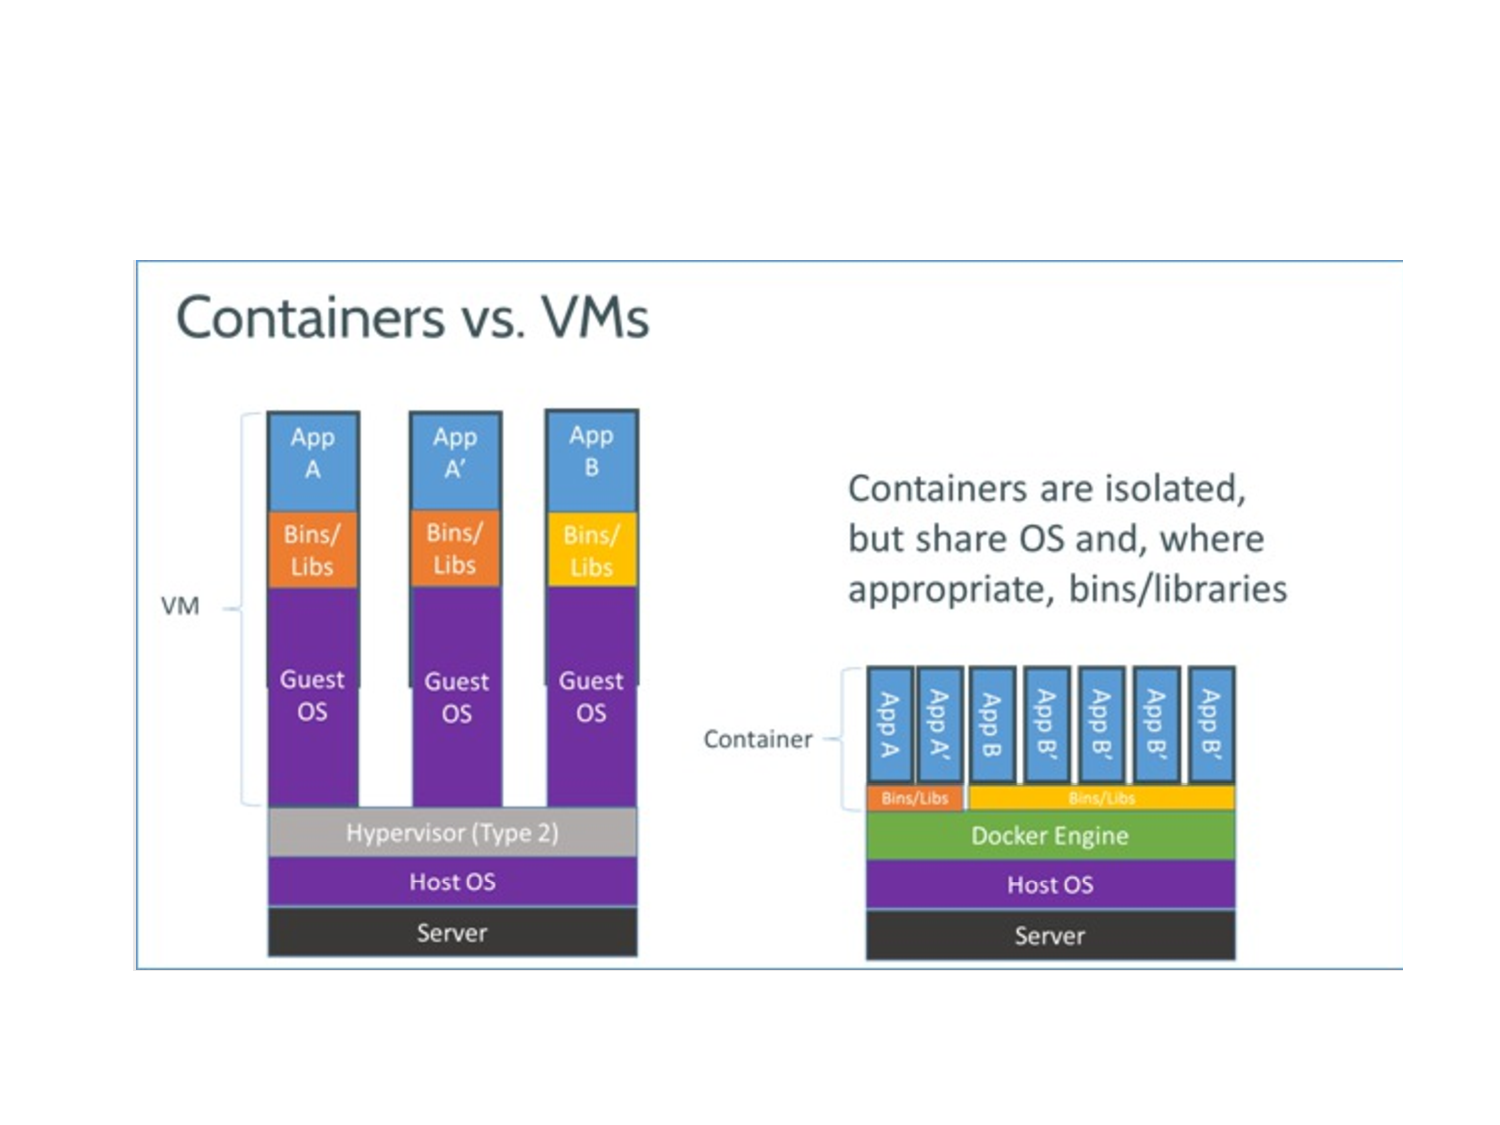
\includegraphics[width=0.8\linewidth]{figs/vm-lxc.pdf}
\end{center}

}

\frame{
  \frametitle{Docker: why ?}
  \begin{block}{}
    \myred{Efficiency:} \emph{almost} no overhead
    \begin{itemize}
      \item processes are isolated but run straight on the host
      \item \texttt{CPU} performance = \myred{native} performance
      \item memory performance = a few \% shaved off for (optional) accounting
      \item network performace = small overhead
    \end{itemize}
  \end{block}

  \begin{block}{}
    \myred{Efficiency:} storage friendly
    \begin{itemize}
      \item unioning filesystems
      \item snapshotting filesystems
      \item copy-on-write
    \end{itemize}
  \end{block}

  \begin{block}{}
    \begin{itemize}
      \item provisionning takes a few milliseconds
      \item \ldots and a few kilobytes
      \item creating a new container/base-image takes a few seconds
    \end{itemize}
  \end{block}
}

%% \frame{
%%   \frametitle{Docker: how ?}

%%   \begin{block}{}
%%     \begin{itemize}
%%       \item LinuX Containers (LXC)
%%       \item Control Groups and Namepsaces
%%       \item AUFS (overlaying filesystem), or BTRFS, or DeviceMapper
%%       \item Client-Server with an \texttt{http/REST} API
%%     \end{itemize}
%%   \end{block}

%%   \begin{block}{LXC}
%%     \begin{itemize}
%%       \item Let's your run a Linux system within another Linux system
%%       \item A container is a group of processes on a Linux box, put together is an isolated environment
%%       \item From the inside, it looks like a VM. From the outside, it looks like normal processes
%%       \item \emph{''chroot on steroids''}
%%     \end{itemize}
%%   \end{block}

%%   \begin{block}{Control Group \& Namespaces}
%%     Linux kernel feature to limit, account and isolate resource usage:
%%     \begin{itemize}
%%       \item CPU
%%       \item Memory
%%       \item disk I/O
%%     \end{itemize}
%%   \end{block}
%% }

\begin{frame}[fragile]
  \frametitle{Docker: introduction}

  \begin{block}{}
    Hello World
    \begin{itemize}
      \item get a base container (ubuntu, centos, \ldots)
\begin{minted}[]{sh}
$ docker pull ubuntu
\end{minted}

      \item list images already pulled in:
\begin{minted}[]{sh}
$ docker images
\end{minted}
\begin{center}
  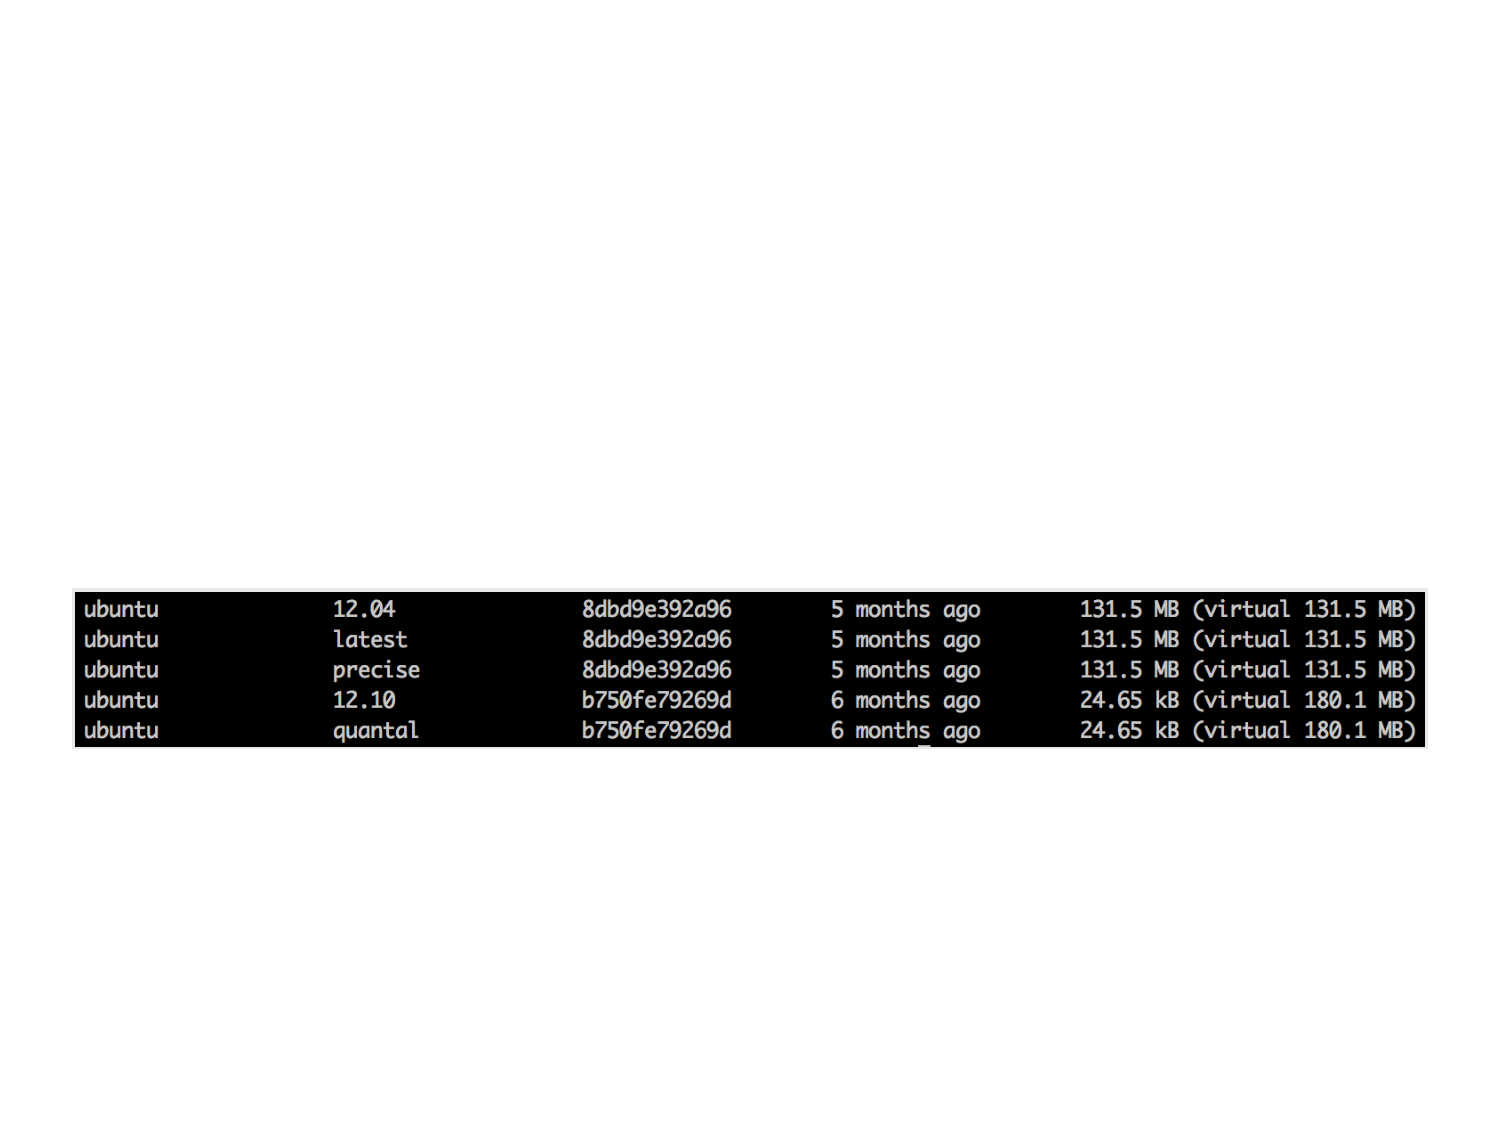
\includegraphics[width=1.0\linewidth]{figs/docker-images.pdf}
\end{center}

      \item run an executable inside a container
\begin{minted}[]{sh}
$ docker run ubuntu:12.10 echo ``hello world''
\end{minted}
    \end{itemize}

  \end{block}
\end{frame}

\begin{frame}[fragile]
  \frametitle{Docker: introduction - II}


\begin{block}{}
  Detached mode
  \begin{itemize}
    \item run a container in detached mode:
\begin{minted}[]{sh}
$ docker run -d ubuntu sh -c \
  while true; do echo ''hello''; sleep 1; done;
\end{minted}

    \item get the container id:
\begin{minted}[]{sh}
$ docker ps
\end{minted}
\begin{center}
  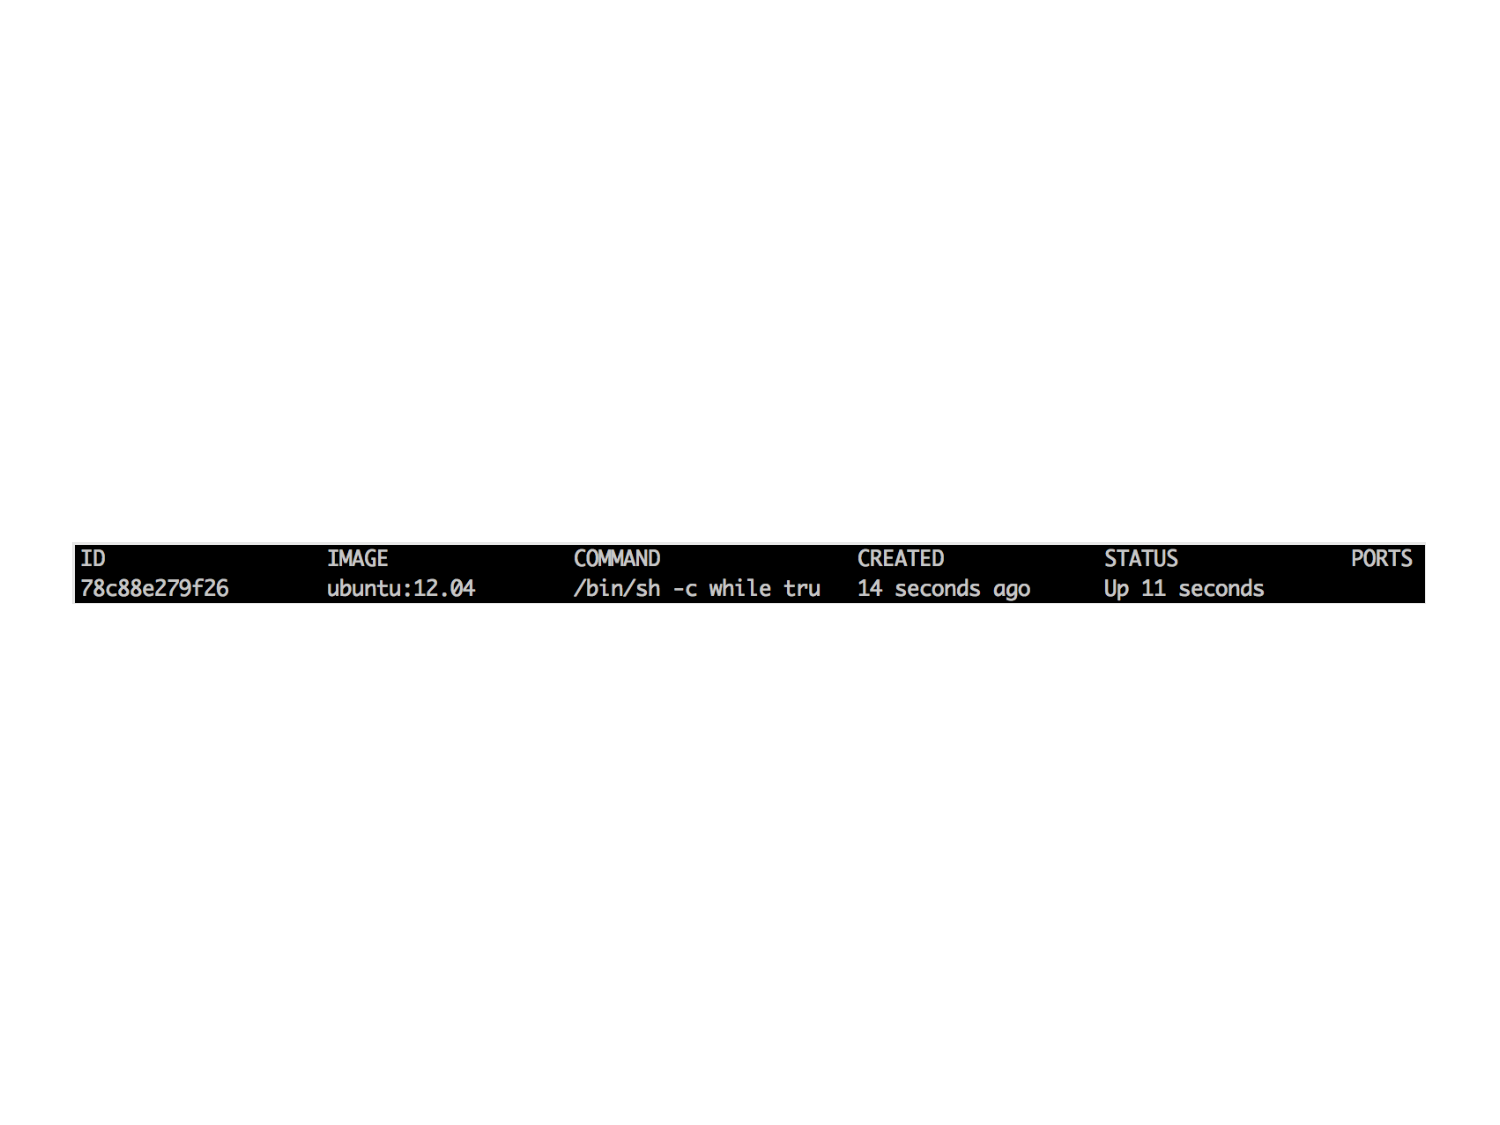
\includegraphics[width=1.0\linewidth]{figs/docker-ps.pdf}
\end{center}

    \item attach to the container
\begin{minted}[]{sh}
$ docker attach 78c88e279f26
\end{minted}

    \item start/stop/restart a container
\begin{minted}[]{sh}
$ docker stop 78c88e279f26
\end{minted}

  \end{itemize}
\end{block}

\end{frame}

\begin{frame}[fragile]
  \frametitle{Docker: public index}
\begin{block}{}
  Public index
  \begin{itemize}
    \item pull an \texttt{apache} container from the index:
\begin{minted}[]{sh}
$ docker search apache
$ docker pull creack/apache2
\end{minted}

\item run the image and check the ports
\begin{minted}[]{sh}
$ docker run -d creack/apache2
$ docker ps
\end{minted}
\begin{center}
  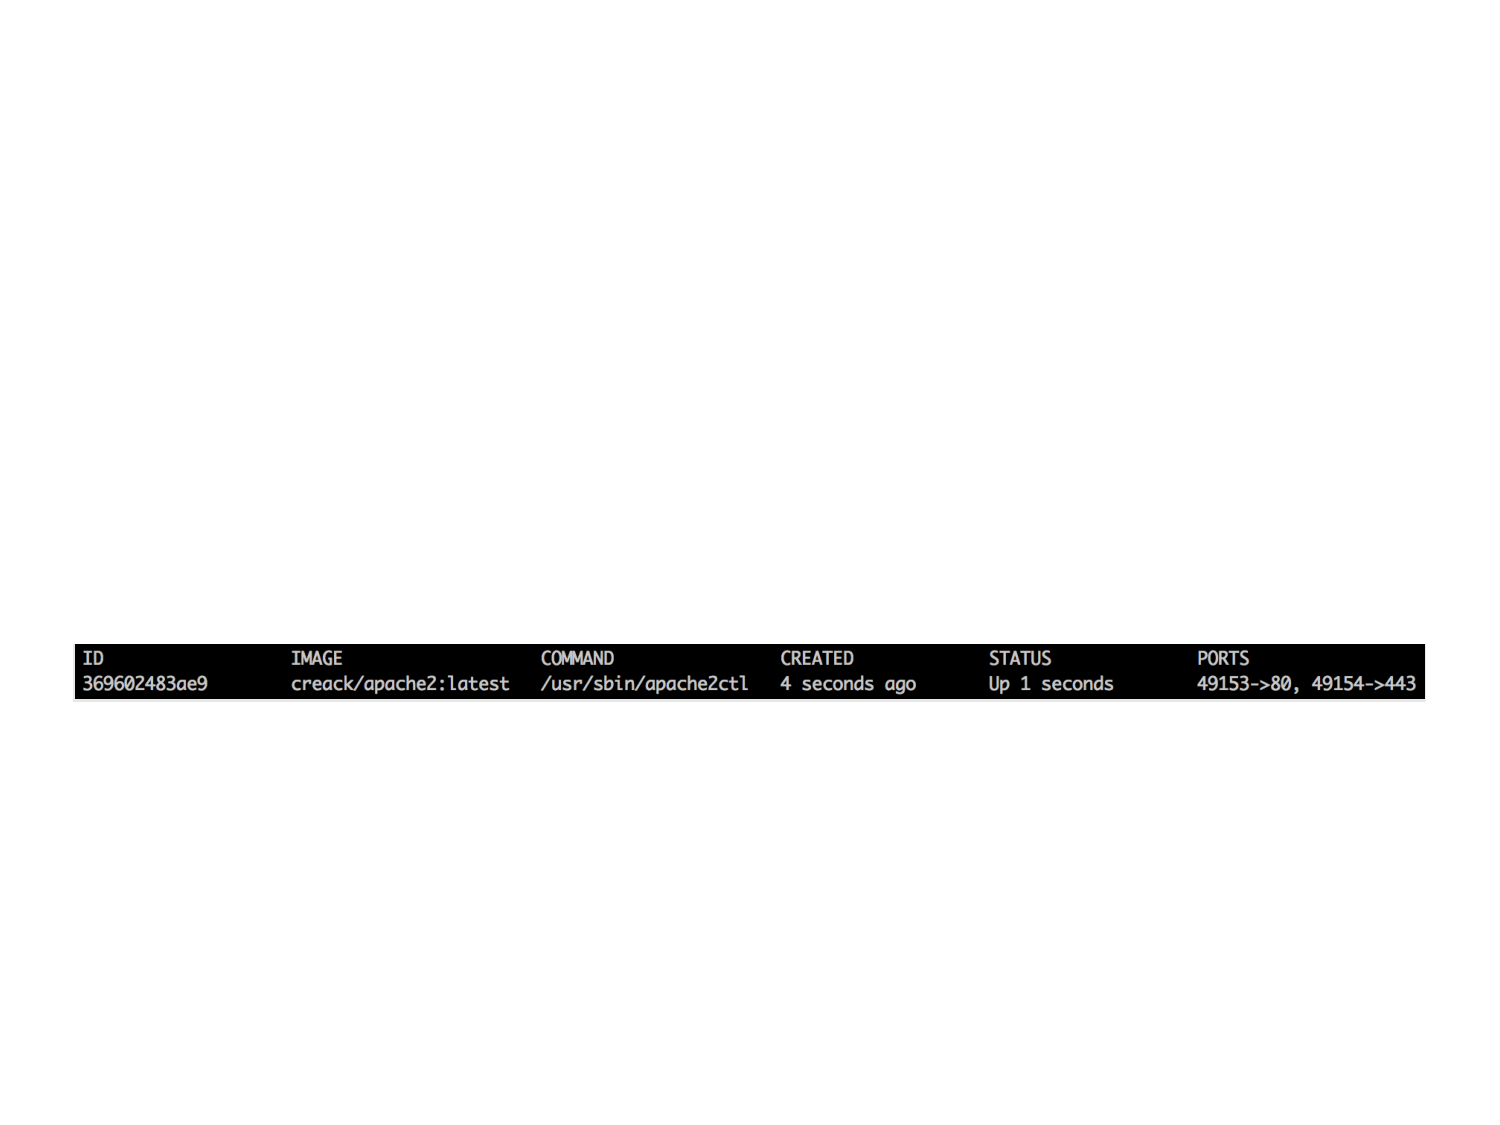
\includegraphics[width=1.0\linewidth]{figs/docker-ps-apache.pdf}
\end{center}
  \end{itemize}
\end{block}

\begin{block}{}
Also available from the browser:\\
\myblue{\href{https://index.docker.io/}{\texttt{https://index.docker.io/}}}
\end{block}

\end{frame}

\begin{frame}[fragile]
  \frametitle{Docker: creating a customized container}
\begin{block}{}
\begin{itemize}
  \item run \texttt{docker} interactively:
\begin{minted}[]{sh}
$ docker run -i -t ubuntu bash
root@bf72b1a06e6c:/# apt-get update
Reading package lists... Done

root@bf72b1a06e6c:/# apt-get install memcached
[...]
root@bf72b1a06e6c:/# exit
\end{minted}

  \item commit the resulting container
\begin{minted}[]{sh}
$ docker commit `docker ps -q -l ` binet/memcached
ab59e4b14266
\end{minted}

  \item run the image
\begin{minted}[]{sh}
$ docker run -d -p 11211 -u daemon binet/memcached memcached
ab59e4b14266
\end{minted}
\end{itemize}
\end{block}
\end{frame}

\begin{frame}[fragile]
  \frametitle{Docker: creating a customized container - Dockerfile}
\begin{block}{}
\begin{minted}[]{sh}
## install gaudi from RPMs
FROM hepsw/slc-base
MAINTAINER binet@cern.ch

ENV MYSITEROOT /opt/lhcb-sw
ENV CMTCONFIG x86_64-slc6-gcc48-opt

RUN mkdir -p $MYSITEROOT

## install some system dependencies
RUN yum install -y bzip2 freetype glibc-headers tar which

## retrieve install
RUN curl -O -L  http://cern.ch/lhcbproject/dist/rpm/lbpkr && \
    chmod +x ./lbpkr

## install (source+binaries)
RUN ./lbpkr install-project GAUDI v26r1
\end{minted}

\end{block}
\end{frame}

\begin{frame}[fragile]
\frametitle{Docker: Dockerfile - II}
\begin{block}{}
\begin{itemize}
  \item build the container
\begin{minted}[]{sh}
$ docker build --tag=hepsw/lhcb-gaudi:v26r1 .
$ docker tag hepsw/lhcb-gaudi:v26r1 hepsw/lhcb-gaudi:latest
\end{minted}
\end{itemize}
\end{block}

\begin{block}{}
\begin{itemize}
  \item run the container (and test the build)
\begin{minted}[]{sh}
$ docker run -i -t hepsw/lhcb-gaudi /bin/bash
[hepsw/lhcb-gaudi] $ cd /scratch
[hepsw/lhcb-gaudi] $ gaudirun.py \
   $GAUDIEXAMPLESROOT/options/TupleEx.py
\end{minted}

 \item bind mounts
\begin{minted}[]{sh}
$ docker run -i -t hepsw/lhcb-gaudi \
  -v /host/build/results:/scratch
  /bin/bash
\end{minted}

 \item copy files from container to host
\begin{minted}[]{sh}
$ docker cp hepsw/lhcb-gaudi:/scratch /host/build/results
\end{minted}

\end{itemize}
\end{block}
\end{frame}

%% \frame{
%%   \frametitle{Docker: when ? where ?}

%% \begin{block}{}
%%   \begin{itemize}
%%     \item \texttt{OpenStack-Havana} has support for running \texttt{docker} containers
%%     \item so since beginning 2014: technically possible to run those on \texttt{openstack.cern.ch} (some configuration required though [\myblue{\href{https://cern.service-now.com/service-portal/view-request.do?n=RQF0335022}{\texttt{RQF0335022}}}])
%%   \end{itemize}
%% \end{block}

%% \begin{block}{}
%%   \begin{itemize}
%%     \item since version \texttt{docker-0.7} no \texttt{AUFS} hard-requirement. multiple backends:
%%       \begin{itemize}
%%         \item BTRFS
%%         \item DeviceMapper
%%       \end{itemize}
%%     \item packaged for \texttt{Fedora-20}
%%     \item available on \texttt{RHEL/SLC-6.5} (\texttt{apt-get install docker-io})
%%   \end{itemize}

%% \begin{center}
%%   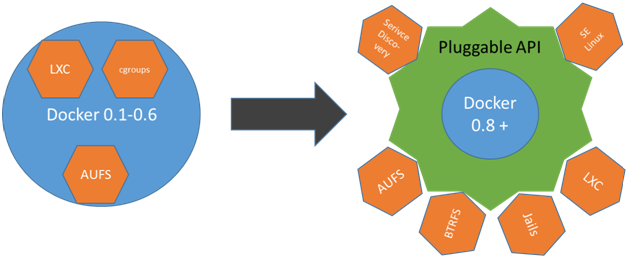
\includegraphics[width=0.7\linewidth]{figs/docker-1.png}
%% \end{center}
%% \end{block}
%% }

\frame{
  \frametitle{Benchmarks}
  \begin{block}{}
    \begin{itemize}
      \item \myblue{\href{http://bodenr.blogspot.ch/2014/05/kvm-and-docker-lxc-benchmarking-with.html}{\texttt{kvm-and-docker-lxc-benchmarking}}}
        \begin{itemize}
          \item \mypurple{executive summary:} \texttt{docker} delivers very close to the bare-metal performances (consistantly better than \texttt{KVM} save for some \texttt{mysql} tests)
        \end{itemize}
      \item tests \texttt{docker} containers creation, guest CPU/Mem/IO performances, \ldots
    \end{itemize}
  \end{block}
}

\begin{frame}[fragile]
  \frametitle{Benchmarks - II}

  \begin{block}{}
    Disk sizes of containers:
        \begin{minted}[]{sh}
REPOSITORY              TAG                 VIRTUAL SIZE
hepsw/lhcb-base         20150331            336.6 MB
hepsw/lhcb-gaudi        v26r1               3.911 GB
hepsw/lhcb-davinci      v36r5               7.790 GB

lhcb-base    (slimmed)  latest              322.3 MB
lhcb-gaudi   (slimmed)  latest              3.893 GB
lhcb-davinci (slimmed)  latest              7.771 GB

hepsw/cvmfs-base        20150331            629.4 MB
hepsw/cvmfs-lhcb        20150331            629.4 MB
        \end{minted}
  \end{block}

  \begin{block}{}
    Disk sizes of \texttt{\$MYSITEROOT}:
    \begin{minted}[]{sh}
hepsw/lhcb-base:    /opt/lhcb-sw    67M
hepsw/lhcb-gaudi:   /opt/lhcb-sw 3.600G
hepsw/lhcb-davinci: /opt/lhcb-sw 7.300G
    \end{minted}
  \end{block}

  \emph{slimmed:} use \texttt{docker export+import} to shrink image size.
\end{frame}

\begin{frame}[fragile]
  \frametitle{Benchmarks - III}

  \begin{block}{}
    Running \texttt{gaudirun.py GaudiExamples/TupleEx.py}
    \begin{itemize}
      \item \texttt{AFS}
        \begin{minted}[]{sh}
56.87s user 14.26s system 66% cpu 1:46.50 total # kick AFS
57.62s user 13.07s system 99% cpu 1:11.17 total
57.69s user 13.46s system 99% cpu 1:11.58 total
57.93s user 13.26s system 99% cpu 1:11.66 total
        \end{minted}

      \item \texttt{Docker-RPMs}
        \begin{minted}[]{sh}
55.93s user 12.34s system 98% cpu 1:09.54 total
55.43s user 12.88s system 98% cpu 1:09.12 total
55.54s user 12.16s system 98% cpu 1:08.83 total
55.39s user 11.60s system 98% cpu 1:07.81 total
        \end{minted}

      \item \texttt{Docker-CVMFs} (a \texttt{docker} container where
        \texttt{CVMFs} is configured and running)
        \begin{minted}[]{sh}
55.53s user 14.01s system 88% cpu 1:18.75 total # kick CVMFs
54.95s user 12.83s system 97% cpu 1:09.36 total
55.42s user 12.86s system 98% cpu 1:09.35 total
55.42s user 13.01s system 98% cpu 1:09.63 total
        \end{minted}

    \end{itemize}
  \end{block}
\end{frame}

\frame{
  \frametitle{Docker: on non-Linux ?}

\begin{block}{}
  \begin{itemize}
    \item no container backend for MacOSX (yet?)
    \item it is foreseen that at some point a \texttt{jail}-based backend will appear
    \item in the meantime: \myblue{\href{http://docs.docker.io/installation/mac/}{\texttt{boot2docker}}}
      \begin{itemize}
        \item launches a very thin Linux-VM where the \texttt{docker} daemon is installed
        \item installs the \texttt{docker} client on the host
        \item talks via HTTP/REST to the daemon
      \end{itemize}
  \end{itemize}
\end{block}

\begin{block}{}
  \begin{itemize}
    \item \texttt{boot2docker} works also for \texttt{Windows (TM)}
  \end{itemize}
\end{block}

}

\frame{
  \frametitle{Conclusions \& Prospects}

\begin{block}{}
  \begin{itemize}
    \item easily distribute dev-environments
    \item easily provision build and dev-environments
    \item easily relocate binaries (remember: \texttt{chroot} on steroids!)
    \item provision efficient performance-wise environments (production)
  \end{itemize}

    \begin{center}
      
\includegraphics[width=0.35\linewidth]{figs/docker-logo.png}
    \end{center}

    \begin{itemize}
      \item run a \texttt{HEP}-dedicated \texttt{docker} images
        repository ?
        \begin{itemize}
          \item  $ACL$s
          \item $O(GB)$ images \ldots
        \end{itemize}
      \item put a \myblue{\href{http://frontier.cern.ch}{\texttt{Frontier}}} server in front ?
    \end{itemize}
\end{block}
}

\frame{
  \frametitle{Docker: HEP examples}

\begin{block}{}
  \myblue{\href{https://github.com/hepsw/docks}{\texttt{hepsw/docks (github)}}}


  \myblue{\href{https://index.docker.io/search?q=hepsw}{\texttt{hepsw/containers (docker public registry)}}}

\end{block}
}

\end{document}


